\documentclass[11pt]{scrartcl}
\usepackage[utf8]{inputenc}
\usepackage{mathtools}
\usepackage{amssymb}

\usepackage{caption}
\usepackage{color}
\usepackage{xcolor}
\usepackage{listings}
\DeclareCaptionFont{white}{\color{white}}
\DeclareCaptionFormat{listing}{\colorbox{gray}{\parbox{\textwidth}{#1#2#3}}}
\captionsetup[lstlisting]{format=listing,labelfont=white,textfont=white}

\usepackage{tikz}
\usetikzlibrary{automata,positioning}

\usepackage{makecell}

\usepackage{changepage}

\title{\textbf{1810 Einsendeaufgabe KE 02}}
\author{Gustavo Nunes Martins}

\begin{document}
	\maketitle
	\section*{Aufgabe 1}
	Dieses Grammatik ist durch die B-Symbol links-rekursiv und nicht für rekursiven Abstieg geeinigt (unendliche loop). Man kann die links-Rekursion durch eine rechts-Rekursion ersetzen:
	
	\begin{center}
	$B \rightarrow yzzBV \mid AwV$
	
	$B' \rightarrow wzV \mid \varepsilon$
	\end{center}
	Die folgenden Syntax-Diagramme helfen, die Parser zu erzeugen. Die entsprechende Implementation ist nebenan:
	\subsection*{S:}
	\begin{minipage}{.4\textwidth}
	
\includegraphics[width=0.4\linewidth]{ke-02/diagram/diagram/S}

	\end{minipage}
	\begin{minipage}{0.6\textwidth}
	\begin{lstlisting}[language=C]		
void CheckS(){
  CheckA();
  if (lookAhead!=$) then
    {error($)}
}
	\end{lstlisting}
	\end{minipage}
	\subsection*{A:}
	\begin{minipage}{0.4\textwidth}
	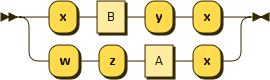
\includegraphics[width=1\linewidth]{ke-02/diagram/diagram/A}
	\end{minipage}
	\begin{minipage}{0.6\textwidth}
		\begin{lstlisting}[language=C]		
bool CheckA(){
  if (lookAhead=='x') then 
    {CheckB();match('y');match('x');return TRUE}
  else if (lookAhead=='w') then 
    {match('z');checkA();match('x');return TRUE}
  else error('A');
}
		\end{lstlisting}
	\end{minipage}	
	\subsection*{B:}
	\begin{minipage}{0.4\textwidth}
	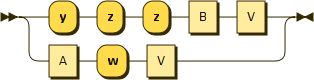
\includegraphics[width=1\linewidth]{ke-02/diagram/diagram/B}
	
	\end{minipage}
	\begin{minipage}{0.6\textwidth}
	\begin{lstlisting}[language=C]		
void CheckB(){
if (lookAhead=='y') then 
  {match('z');match('z');checkB();checkV();}
else if (checkA()) then 
  {match('w');checkV();}
else error('B');
}
\end{lstlisting}
	\end{minipage}
	\subsection*{V:}
	\begin{minipage}{0.4\textwidth}
	
\includegraphics[width=1\linewidth]{ke-02/diagram/diagram/V}
	\end{minipage}
	\begin{minipage}{0.6\textwidth}
		\begin{lstlisting}[language=C]		
void CheckV(){
  if (lookAhead=='w') then 
    {match('z');checkV();}
  else {}
}
		\end{lstlisting}
	\end{minipage}
\begin{lstlisting}[language=C]

int main(){
  lookAhead = nextSymbol();
  checkS();
}
		
void match(terminal t){
  if lookAhead != t then 
    error(t);
  else
    {lookAhead = nextSymbol();} / nextSymbol aus den Lexer
}

void error(symbol failedOn){
  printf("ERROR: Symbol %s malformed\n", failedOn);
  exit(-1);
}

\end{lstlisting}
	\section*{Aufgabe 2}
	\subsection*{a}
	Nur 2 Produktionsregeln sind verändert, nämlich:

	\begin{tabular}{l|l}
		vorher & naher \\ \hline
		$S \rightarrow aTbUcU \mid aTbU$ & 
		\makecell{$S \rightarrow aTbUS'$\\$ S'\rightarrow cU\mid \varepsilon$}
		\\ \hline
		$T\rightarrow dVd \mid dVdW \mid dVdX$ & \makecell{$T\rightarrow dVdT'$ \\$ T'\rightarrow \varepsilon\mid W \mid X$}
	\end{tabular}
	\subsection*{b}

		Folgende Bild erklärt die Herleitung des Folowmenge, wobei FLW(A) bedeutet FOLLOW(A) und FSME(A) bedeutet FIRST(A) - $ \{\varepsilon\} $
		\newline
		\newline
		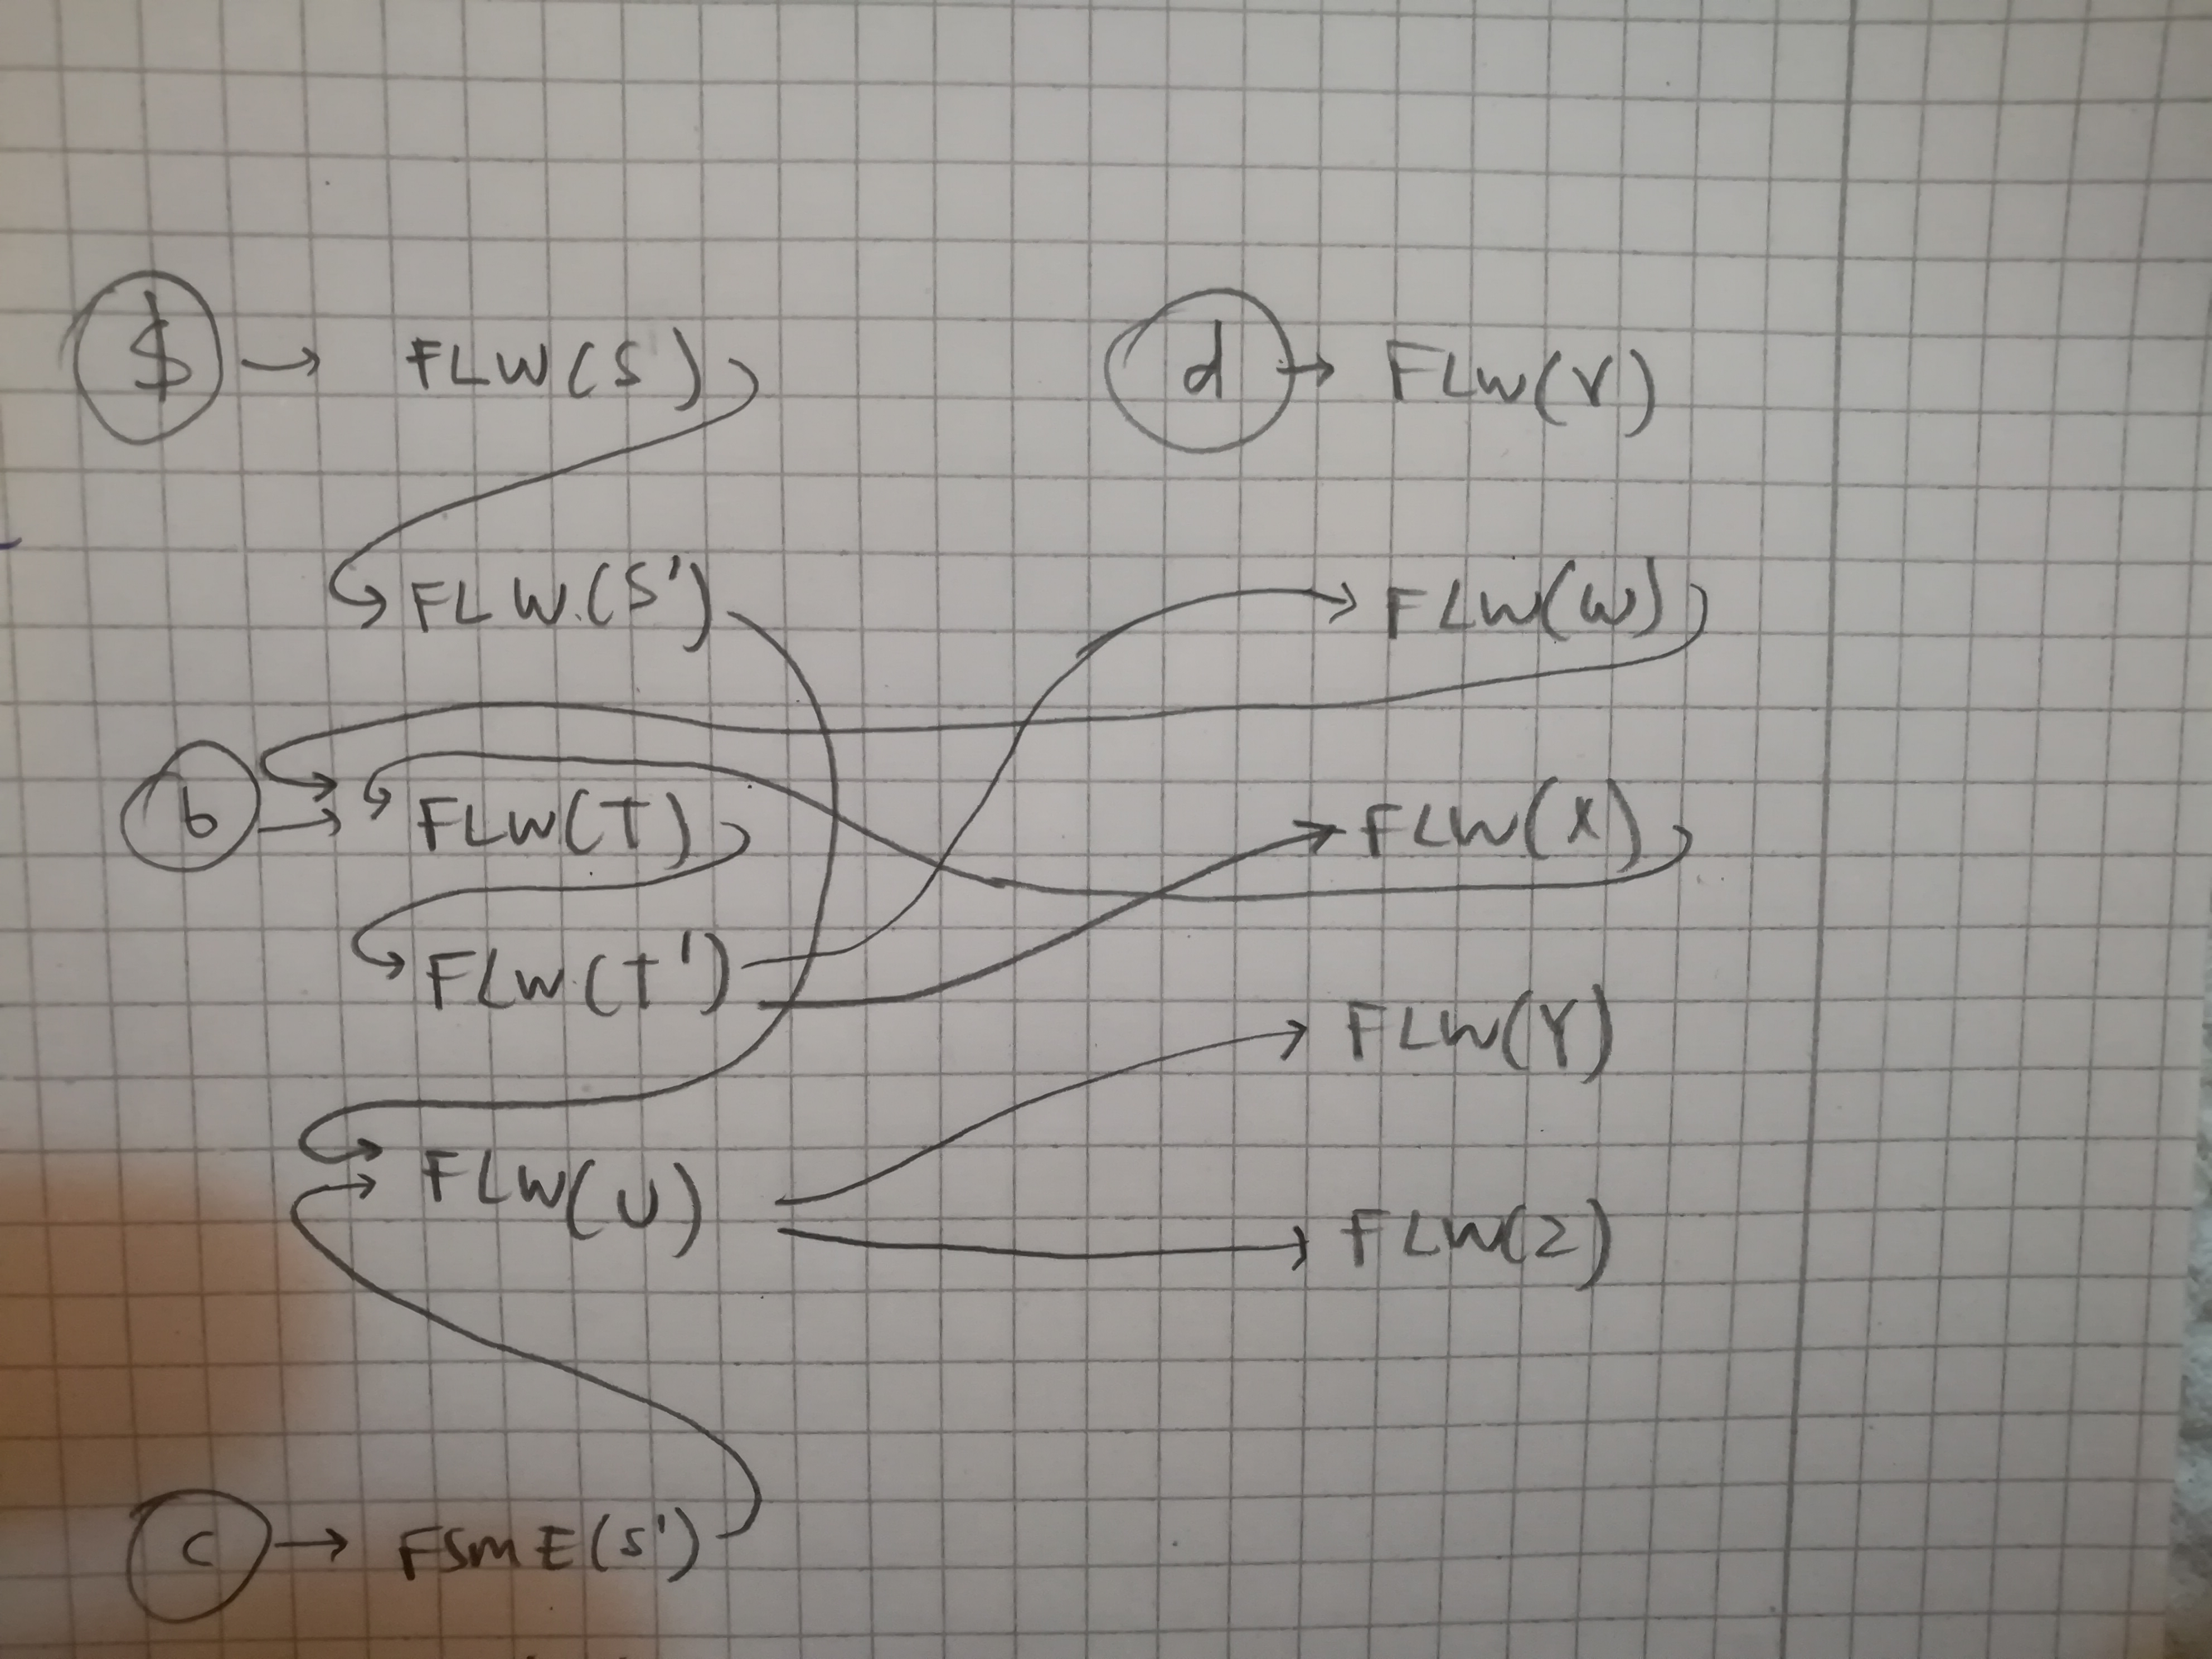
\includegraphics[width=0.7\linewidth]{followset}
		\newline
		An dieser Bild, \$ gehort zum FLW(S) (gezeigt durch die von den link Seite ankommende Pfeil), und alle Elemente von FLW(S) gehören zum FLW(S'). Die richttung eines Pfeil bestimmt die zurehorigkeit zwischen Mengen. Alle elementen von FLW(S') gehören auch zum FLW(U), und alle Elementen von FSME(S') gehoren zum FLW(U) Das erbigt folgende FIRST und FOLLOW Mengen:
		\newline
		\newline
	\begin{tabular}{l|l|l}
		Regel & FIRST & FOLLOW \\ \hline
		S & \{a\} & \{\$\}  \\
		S' & $\{\varepsilon,c\}$ & \{\$\}  \\
		T & \{d\} & \{b\}   \\
		T' & $\{\varepsilon,e,f\}$ & \{b\}   \\
		U & $\{h, g, \varepsilon\}$ & \{\$,c\} \\
		V & \{d\} & \{d\} \\
		W & \{e\} & \{b\} \\
		X & \{f\} & \{b\} \\
		Y & \{h\} & \{\$,c\} \\
		Z & $\{g,\varepsilon\}$ & \{\$,c\} 
	\end{tabular}
	\newline


	Für die Steuermenge, FSME(A) bedeutet FIRST(A) - $ \{\varepsilon\}$:
	
	\begin{tabular}{l|l|l}
		Regel & Steuer & Herleitung\\ \hline
		$ S \rightarrow aTbuS'$ 		& $\{a\}$ 		& FIRST(A) \\ \hline
		$ S' \rightarrow cU $ 			& $\{c\}$ 		& FIRST(S') \\
		$ S' \rightarrow \varepsilon $ 	& $\{\$\}$ 		& FOLLOW(S') \\ \hline 
		$ T \rightarrow dVdT' $ 		& $\{d\}$ 		& FIRST(T) \\ \hline
		$ T' \rightarrow W $ 			& $\{e\}$ 		& FIRST(W) \\
		$ T' \rightarrow X $ 			& $\{f\}$ 		& FIRST(X) \\
		$ T' \rightarrow \varepsilon $ 	& $\{b\}$ 		& FOLLOW(T') \\ \hline
		$ U \rightarrow Y $ 			& $\{h\}$ 		& FIRST(Y) \\
		$ U \rightarrow Z $ 			& $\{c,g,\$\}$ 	& FSME(Z) $ \bigcup FOLLOW(Z) $ \\ \hline
		$ V \rightarrow d $ 			& $\{d\}$ 		& FIRST(V) \\ \hline
		$ W \rightarrow eT $ 			& $\{e\}$ 		& FIRST(W) \\ \hline
		$ X \rightarrow fT $ 			& $\{f\}$ 		& FIRST(X) \\ \hline
		$ Y \rightarrow hZ $ 			& $\{h\}$ 		& FIRST(Y) \\ \hline
		$ Z \rightarrow g $ 			& $\{g\}$ 		& FIRST(Z) \\
		$ Z \rightarrow \varepsilon $ 	& $\{c,\$\}$ 	& FOLLOW(Z) \\
	\end{tabular}
	
	\subsection*{c}
	\begin{adjustwidth}{-2cm}{}
	\begin{tabular}{l|l|l|l|l|l|l|l|l|l}
		 & a & b & c & d & e & f & g & h & \$ \\
		S & $ S \rightarrow aTbUS' $ & & & & & & &\\ \hline
		S' & & & $ S' \rightarrow cU $ & & & & & & $ S' \rightarrow \varepsilon $\\ \hline
		T & & & & $ T \rightarrow dVdT' $ & & & &\\ \hline
		T' & & $ T' \rightarrow \varepsilon $ & & & $ T' \rightarrow W $ & $ T' \rightarrow X $ & &\\ \hline
		U & & & $ U \rightarrow Z $ & & & & $ U \rightarrow Z $ & $ U \rightarrow Y $ & $ U \rightarrow Z $\\ \hline
		V & & & & $ V \rightarrow d $ & & & &\\ \hline
		W & & & & & $ W \rightarrow eT $ & & &\\ \hline
		X & & & & & & $ X \rightarrow fT $ & &\\ \hline
		Y & & & & & & & & $ Y \rightarrow hZ $\\ \hline
		Z & & & $ Z \rightarrow \varepsilon $ & & & & $ Z \rightarrow g $ & & $ Z \rightarrow \varepsilon $\\ \hline
	\end{tabular}
	\end{adjustwidth}
	\section*{Aufgabe 3}
	In .zip Datei verfügbar
\end{document}